\section{Model Comparison \& Conclusions}

\begin{frame}{Model Comparison: Trajectories}
    A visual comparison of the stress trajectories and the resulting spin velocity reveals the fundamental differences between the models.

    \begin{figure}
        \centering
        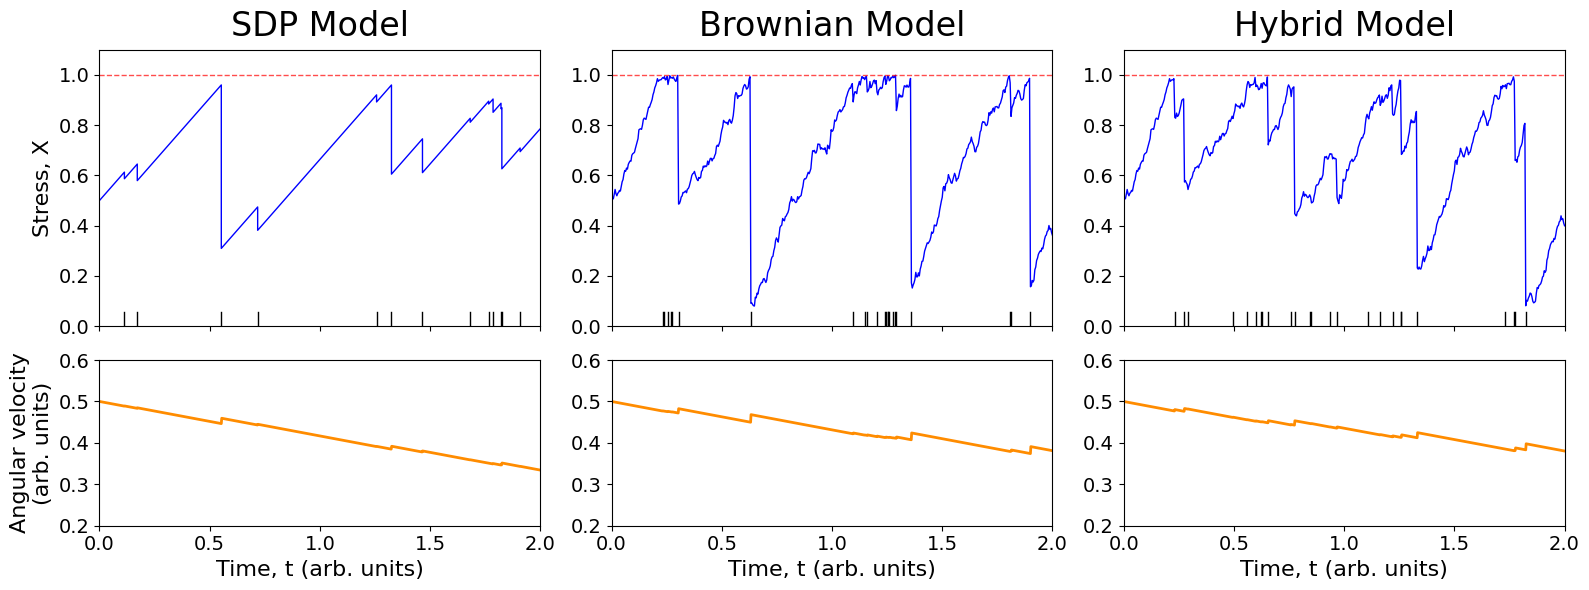
\includegraphics[width=\linewidth]{assets/comparison.png}
    \end{figure}
    
    \vspace{-1em}

    \begin{itemize}
        \item \textbf{SDP Model:} Deterministic, linear ramps with probabilistic triggers.
        \item \textbf{Brownian Model:} Stochastic ramps up to a hard threshold.
        \item \textbf{Hybrid Model:} Stochastic ramps with probabilistic triggers, showing intermediate behavior.
    \end{itemize}
\end{frame}

\begin{frame}{Model Comparison: Key Predictions}
    \centering
    The three models offer distinct predictions for observable glitch statistics.

    \vspace{0.5em}

    \begin{adjustbox}{width=1\textwidth}
    \renewcommand{\arraystretch}{1.5} % increase row height for better vertical centering
    \begin{tabular}{l >{\centering\arraybackslash}m{3.5cm} >{\centering\arraybackslash}m{3.5cm} >{\centering\arraybackslash}m{3.5cm}}
        \toprule
        \rowcolor{gray!15}
        \textbf{Feature} & \textbf{SDP Model} & \textbf{Brownian Model} & \textbf{Hybrid Model} \\
        \midrule
        \textbf{Stress Evolution} & Deterministic & Stochastic (SDE) & Stochastic (SDE) \\
        \rowcolor{gray!10}
        \textbf{Glitch Trigger} & Stochastic Rate $\lambda(X)$ & Deterministic Threshold $X_c$ & Stochastic Rate $\lambda(X)$ \\
        \textbf{Waiting Time PDF} & Power-law (low $\alpha$) or Exponential (high $\alpha$) & Log-Normal / Gaussian (high $\mu$) or Exponential (low $\mu$) & Complex interplay of all parameters \\
        \rowcolor{gray!10}
        \textbf{Correlations} & Predicts backward correlations for some $\eta(\Delta X)$ & Predicts strong forward correlations for high $\mu$ & Potentially rich correlation structure \\
        \bottomrule
    \end{tabular}
    \end{adjustbox}

    \vspace{0.5em}

    \small The hybrid model bridges the gap, allowing for a more nuanced exploration of the underlying physics.
\end{frame}

\begin{frame}{Conclusions}

    \setlength{\leftmargini}{1em}
    \begin{itemize}
        \item The \textbf{Brownian} and \textbf{SDP} models offer two contrasting approaches: noisy stress buildup vs.\ probabilistic failure.
        \item Both explain some observed statistics, but the stress release law $\eta(\Delta X)$ is especially important for the Brownian model.
        \item The \textbf{Hybrid Model} unifies both ideas, combining noise and probabilistic triggering for greater flexibility in modeling real data.
    \end{itemize}
    
    \textbf{Future Work:}
    \begin{itemize}
        \item A systematic analysis of the Hybrid model's parameter space.
        \item Direct comparison of all three models' predictions (e.g., correlation functions) with observational data from pulsar glitch catalogs.
    \end{itemize}
\end{frame}